\section{User Interface}

The user interface was implemented using the lightweight Flask web framework and integrated with a MySQL database. The web app provides a user with the ability to query data for a given node and time range. The data is presented on a plot and can be downloaded as a csv file. The graphics for plotting are provided by Python's \emph{matplotlib} library. The logic to consolidate data for a given time range and scale the plot graphic accordingly is performed by the web app backend.

The interface is a single page broken into four sections, the profile of the selected node which displays relevant information to that end, the live video feed of the selected node and the count and speed statistics for the selected node and datetime range. Figure \ref{fig:dragonfly} shows the individual panes of the web app and web apps the overall appearance.

\begin{figure}[H]
	\centering
    \begin{subfigure}[b]{0.5\linewidth}
        \centering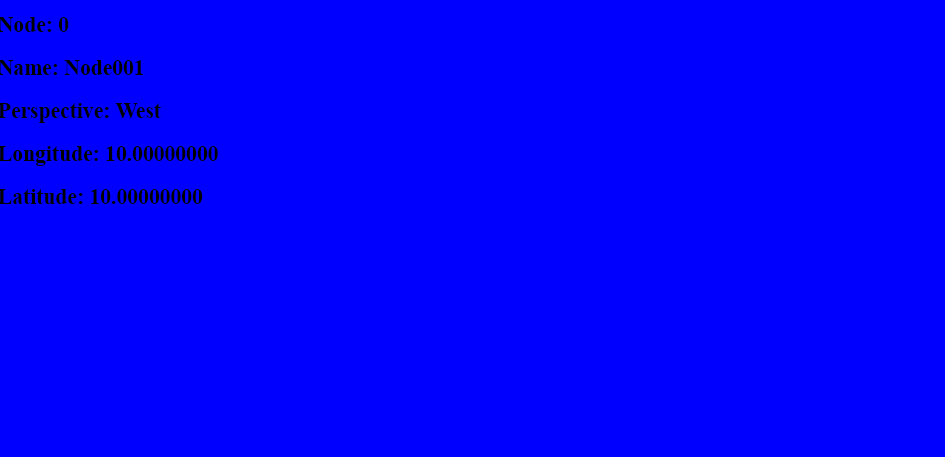
\includegraphics[width = \textwidth]{design/ui/profile}
        \caption{Node Profile}
        \label{fig:}
    \end{subfigure}%
    \begin{subfigure}[b]{0.5\linewidth}
        \centering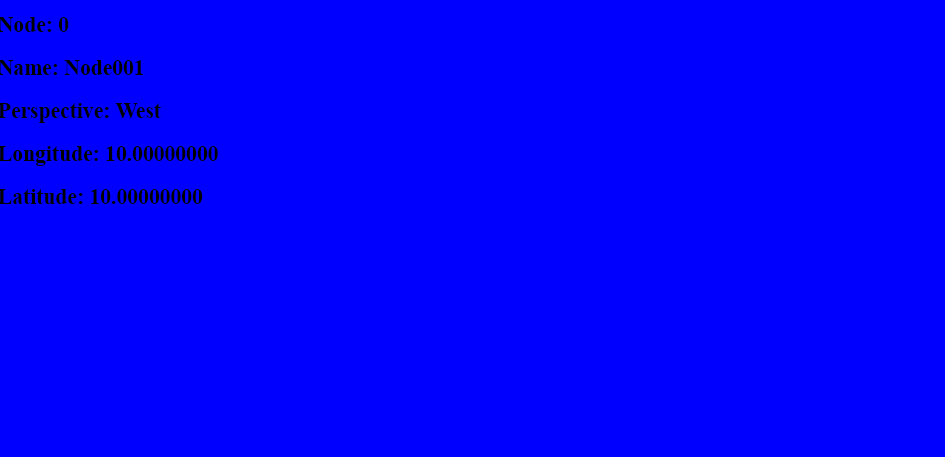
\includegraphics[width = \textwidth]{design/ui/profile}
        \caption{Live Video Feed}
        \label{fig:}
    \end{subfigure}
    \begin{subfigure}[b]{0.5\linewidth}
        \centering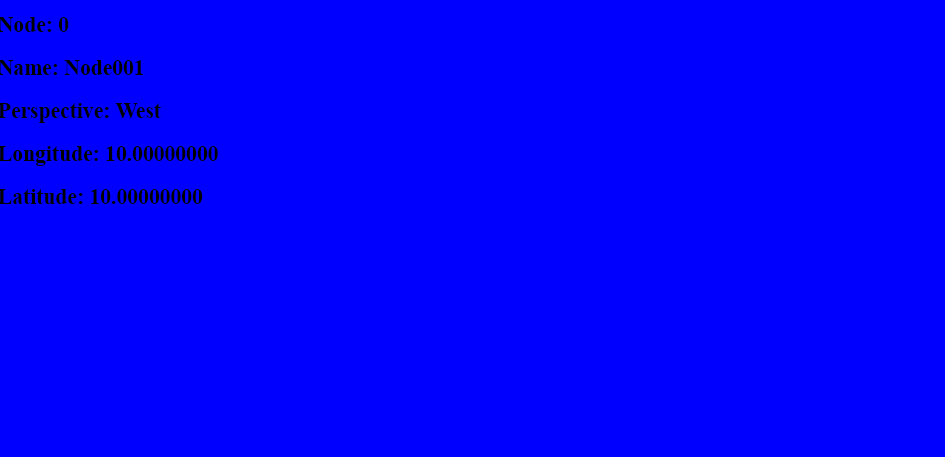
\includegraphics[width = \textwidth]{design/ui/profile}
        \caption{Vehicle Volume Plot}
        \label{fig:}
    \end{subfigure}
    \begin{subfigure}[b]{0.5\linewidth}
        \centering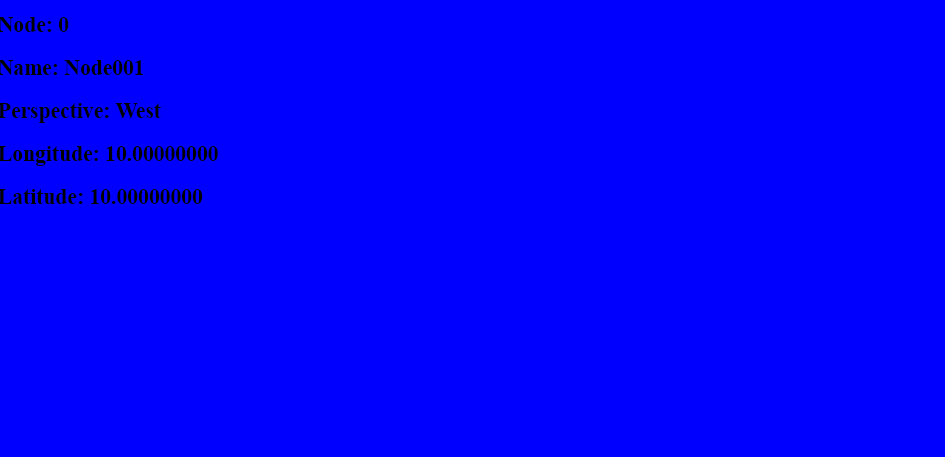
\includegraphics[width = \textwidth]{design/ui/profile}
        \caption{Vehicle Speed Plot}
        \label{fig:}
    \end{subfigure}
    \begin{subfigure}[b]{0.5\linewidth}
        \centering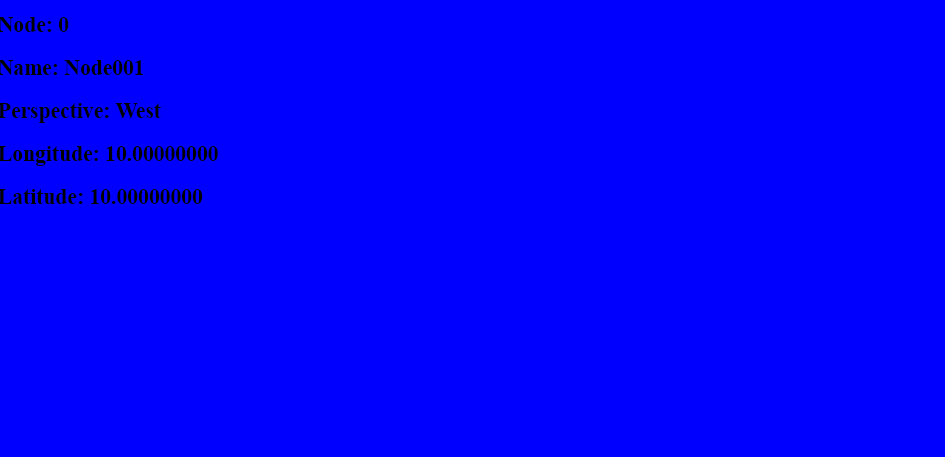
\includegraphics[width = \textwidth]{design/ui/profile}
        \caption{Whole Page View}
            \label{fig:}
    \end{subfigure}
    	\caption{Web Application - User Interface Panes}
    	\label{fig:dragonfly}
\end{figure}


